The single asset test cases are designed to test the basic elements of the classical-PSHA based risk calculator, such as:

\begin{itemize}
\item asset loss ratio exceedance curve computation
\item asset loss exceedance curve computation
\end{itemize}

The location and taxonomy of the single asset in the exposure model used for the single-asset test cases for the classical risk calculator are given in Table~\ref{tab:asset}.

% ---------------------------------------------------------------------------
\subsubsection{Case 1a}
Table~\ref{tab:vf-ln-tax1-zcov} shows the mean loss ratios and corresponding coefficients of variation for the vulnerability function used in this test case.

When the exposure model and vulnerability model are provided to the OpenQuake classical PSHA-based hazard calculator, OpenQuake computes the hazard curves at the locations of the assets in the exposure model and at the specific intensity levels used in the vulnerability functions.

\begin{table}[htbp]

\centering
\tabcolsep=0.11cm
\scalebox{0.6}{

\begin{tabular}{ l c c c c c c c c c c c }

\hline
\rowcolor{anti-flashwhite}
\bf{PGA} & \bf{0.05g} & \bf{0.20g} & \bf{0.40g} & \bf{0.60g} & \bf{0.80g} & \bf{1.00g} & \bf{1.20g} & \bf{1.40g} & \bf{1.60g} & \bf{1.80g} & \bf{2.00g} \\
\hline
\bf{P.O.E.} & 3.896\times10^{-2} & 2.222\times10^{-2} & 8.171\times10^{-3} & 3.070\times10^{-3} & 1.230\times10^{-3} & 5.195\times10^{-4} & 2.254\times10^{-4} & 9.918\times10^{-5} & 4.353\times10^{-5} & 1.830\times10^{-5} & 6.925\times10^{-6} \\
\hline
\end{tabular}

}

\caption{Hazard curve for PGA at a single site}
\label{tab:hc-l1}
\end{table}

The intensity levels for the hazard curve are extracted from the vulnerability function: $[0.05, 0.20, 0.40, 0.60, 0.80, 1.00, 1.20, 1.40, 1.60, 1.80, 2.00]$. The hazard curve gives the probabilities of exceedance for a set of intensity levels within a specified time period. The time period in this case, $t_H$, is one year. The hazard curve at the location of the single asset used in this test case is shown in Table~\ref{tab:hc-l1}.

The probabilities of exceedance are: $[3.896\times10^{-2}, 2.222\times10^{-2}, 8.171\times10^{-3}, 3.070\times10^{-3}, 1.230\times10^{-3}, 5.195\times10^{-4}, 2.254\times10^{-4}, 9.918\times10^{-5}, 4.353\times10^{-5}, 1.830\times10^{-5}, 6.925\times10^{-6}]$. The probabilities of exceedance are first converted to annual rates (or frequencies) of exceedance by employing the Poissonion conversion:

\begin{equation}
	\lambda(iml) = \frac{-\ln [1 - prob(IML > iml, t_H)]}{t_H}
\end{equation}

The annual frequencies of exceedance are: $[3.974\times10^{2}, 2.247\times10^{2}, 8.205\times10^{3}, 3.075\times10^{3}, 1.231\times10^{3}, 5.197\times10^{4}, 2.254\times10^{4}, 9.918\times10^{5}, 4.353\times10^{5}, 1.829\times10^{5}, 6.925\times10^{6}]$.

The annual frequencies of occurrence are estimated by the differentiation of the annual frequencies of exceedance: $[1.727\times10^{2}, 1.426\times10^{2}, 5.130\times10^{3}, 1.845\times10^{3}, 7.109\times10^{4}, 2.942\times10^{4}, 1.262\times10^{4}, 5.565\times10^{5}, 2.524\times10^{5}, 1.137\times10^{5}]$.

The loss ratios at which the loss curve exceedance probabilities are calculated are obtained from the vulnerability function and the parameter `steps\_per\_interval'. The default value of `steps\_per\_interval' is one, which is the value used in this case. The loss ratios in the vulnerability function are $[0.01, 0.04, 0.10, 0.20, 0.33, 0.50, 0.67, 0.80, 0.90, 0.96, 0.99]$.

The vulnerability model is then transformed into a matrix describing probabilities of exceedance for the selected set of loss ratios conditional on the set of ground motion intensity levels. Since there is no variability in the loss ratio, calculation of the loss curves is straightforward in this case. Since the coefficients of variation in the vulnerability function are all zero, the lognormal distribution devolves into the degenerate distribution. The loss ratio exceedance matrix in this case is shown in Table~\ref{tab:lrem-ln-tax1-zcov}.

\begin{table}[htbp]

\centering
\begin{tabular}{ l c c c c c c c c c }

\hline
\rowcolor{anti-flashwhite}
\bf{LR | PGA} & \bf{0.05g} & \bf{0.20g} & \bf{0.40g} & \bf{0.60g} & \bf{0.80g} & \bf{1.00g} & \bf{1.20g} & \bf{\dots} & \bf{2.00g} \\
\hline
\bf{0.01} & 1 & 1 & 1 & 1 & 1 & 1 & 1 & \dots & 1 \\
\bf{0.04} & 0 & 1 & 1 & 1 & 1 & 1 & 1 & \dots & 1 \\
\bf{0.10} & 0 & 0 & 1 & 1 & 1 & 1 & 1 & \dots & 1 \\
\bf{0.20} & 0 & 0 & 0 & 1 & 1 & 1 & 1 & \dots & 1 \\
\bf{0.33} & 0 & 0 & 0 & 0 & 1 & 1 & 1 & \dots & 1 \\
\bf{0.50} & 0 & 0 & 0 & 0 & 0 & 1 & 1 & \dots & 1 \\
\bf{0.67} & 0 & 0 & 0 & 0 & 0 & 0 & 1 & \dots & 1 \\
\bf{0.80} & 0 & 0 & 0 & 0 & 0 & 0 & 0 & \dots & 1 \\
\bf{0.90} & 0 & 0 & 0 & 0 & 0 & 0 & 0 & \dots & 1 \\
\bf{0.96} & 0 & 0 & 0 & 0 & 0 & 0 & 0 & \dots & 1 \\
\bf{0.99} & 0 & 0 & 0 & 0 & 0 & 0 & 0 & \dots & 1 \\
\bf{1.00} & 0 & 0 & 0 & 0 & 0 & 0 & 0 & \dots & 0 \\
\hline
\end{tabular}

\caption{Conditional loss ratio exceedance matrix for classical risk test case 1a}
\label{tab:lrem-ln-tax1-zcov}
\end{table}

Now, the sum product of each row of the conditional loss ratio exceedance matrix with the annual frequencies of occurrence of the respective intensity levels gives the annual frequency of exceedance for the respective loss ratios. The loss ratio annual frequencies of exceedance thus calculated are: $[3.973\times10^{2}, 3.110\times10^{2}, 1.533\times10^{2}, 5.633\times10^{3}, 2.146\times10^{3}, 8.682\times10^{4}, 3.656\times10^{4}, 1.554\times10^{4}, 6.443\times10^{5}, 2.399\times10^{5}]$.

The probabilities of exceedance of the set of loss ratios are obtained by converting the frequencies of exceedance back into probabilities by using the Poissonion assumption. The loss curve probabilities of exceedance are: $[3.895\times10^{2}, 3.062\times10^{2}, 1.521\times10^{2}, 5.617\times10^{3}, 2.144\times10^{3}, 8.678\times10^{4}, 3.655\times10^{4}, 1.554\times10^{4}, 6.443\times10^{5}, 2.399\times10^{5}, 5.683\times10^{6}]$.

The loss curve thus calculated above is compared with the loss curve obtained using the OpenQuake classical PSHA based risk calculator in Figure~\ref{fig:lc-cr-1a}.

\begin{figure}[htbp]
\centering
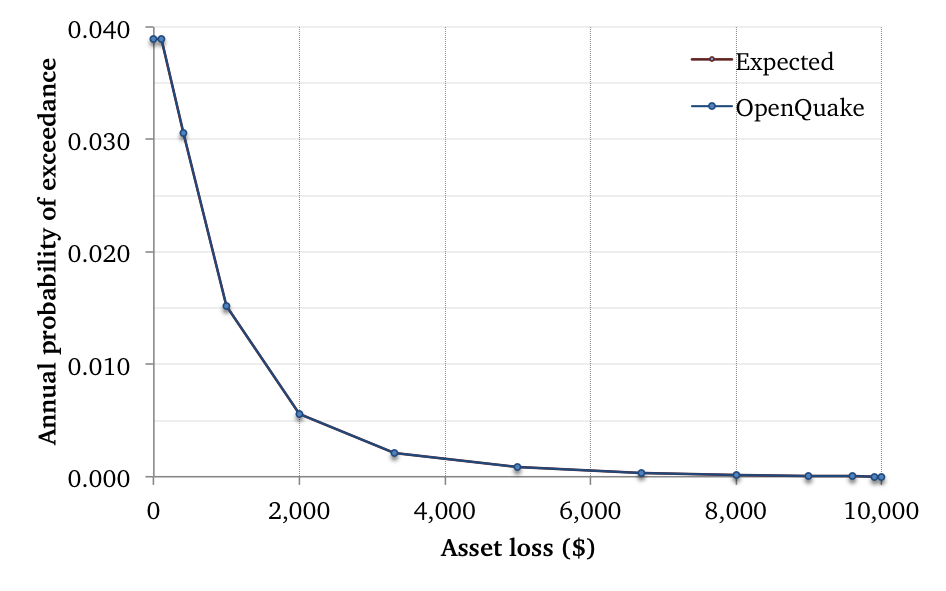
\includegraphics[width=12cm]{qareport/figures/fig-lc-cr-1a}
\caption{Loss curve comparison for classical risk test case 1a}
\label{fig:lc-cr-1a}
\end{figure}

The area under the annual loss exceedance curve gives the average annual loss.

\begin{table}[htbp]

\centering
\begin{tabular}{ l r r r }

\hline
\rowcolor{anti-flashwhite}
\bf{Result} & \bf{Expected} & \bf{OpenQuake} & \bf{Difference}\\
\hline
Average loss & 59.70 & 59.70 & 0\% \\
\hline
\end{tabular}

\caption{Results for classical risk test case 1a}
\label{tab:result-classical-risk-1a}
\end{table}
Table~\ref{tab:result-cr-1a} shows the comparison of the OpenQuake result for average annual loss with the expected result.

% % ---------------------------------------------------------------------------
\subsubsection{Case 1b}
This test case is identical to Case~1a described above, except for the use of the Beta distribution for the vulnerability functions instead of the lognormal distribution. Since the coefficients of variation in the vulnerability function are all zero, once again the Beta distribution devolves into the degenerate distribution as in the previous case. The results for this test case should be exactly the same as in Case~1a.
\begin{table}[htbp]

\centering
\begin{tabular}{ l r r r }

\hline
\rowcolor{anti-flashwhite}
\bf{Result} & \bf{Expected} & \bf{OpenQuake} & \bf{Difference}\\
\hline
Average loss & 45.55 & 45.55 & 0\% \\
\hline
\end{tabular}

\caption{Results for classical risk test case 1b}
\label{tab:result-cr-1b}
\end{table}
Table~\ref{tab:result-cr-1b} shows the comparison of the OpenQuake result for average annual loss with the expected result.

% % % ---------------------------------------------------------------------------
\subsubsection{Case 1c}
This test case repeats the exercise from Case~1a using a vulnerability model with nonzero coefficients of variation. Table~\ref{tab:vf-ln-tax1-nzcov} shows the mean loss ratios and corresponding coefficients of variation for the vulnerability function used in this test case.

Apart from the computation of the conditional loss ratio exceedance matrix, the steps for computing the loss exceedance curve in this case are the same as those employed in Case~1a. The conditional loss ratio exceedance matrix in this case is populated by evaluating the complementary cumulative distribution function (CCDF) of the lognormal distribution at each of the prescribed intensity levels, for the set of loss ratios.

\begin{table}[htbp]

\centering
\begin{tabular}{ l c c c c c c c c c }

\hline
\rowcolor{anti-flashwhite}
\bf{LR | PGA} & \bf{0.05g} & \bf{0.20g} & \bf{0.40g} & \bf{0.60g} & \bf{0.80g} & \bf{1.00g} & \bf{1.20g} & \bf{\dots} & \bf{2.00g} \\
\hline
\bf{0.01} & 0.494 & 1.000 & 1.000 & 1.000 & 1.000 & 1.000 & 1.000 & \dots & 1.000 \\
\bf{0.04} & 0.000 & 0.476 & 1.000 & 1.000 & 1.000 & 1.000 & 1.000 & \dots & 1.000 \\
\bf{0.10} & 0.000 & 0.000 & 0.453 & 0.980 & 0.999 & 1.000 & 1.000 & \dots & 1.000 \\
\bf{0.20} & 0.000 & 0.000 & 0.001 & 0.438 & 0.881 & 0.986 & 0.999 & \dots & 1.000 \\
\bf{0.33} & 0.000 & 0.000 & 0.000 & 0.039 & 0.427 & 0.812 & 0.959 & \dots & 1.000 \\
\bf{0.50} & 0.000 & 0.000 & 0.000 & 0.001 & 0.094 & 0.424 & 0.730 & \dots & 1.000 \\
\bf{0.67} & 0.000 & 0.000 & 0.000 & 0.000 & 0.017 & 0.170 & 0.427 & \dots & 1.000 \\
\bf{0.80} & 0.000 & 0.000 & 0.000 & 0.000 & 0.005 & 0.079 & 0.253 & \dots & 1.000 \\
\bf{0.90} & 0.000 & 0.000 & 0.000 & 0.000 & 0.002 & 0.043 & 0.162 & \dots & 0.999 \\
\bf{0.96} & 0.000 & 0.000 & 0.000 & 0.000 & 0.001 & 0.030 & 0.122 & \dots & 0.844 \\
\bf{0.99} & 0.000 & 0.000 & 0.000 & 0.000 & 0.001 & 0.025 & 0.106 & \dots & 0.494 \\
\bf{1.00} & 0.000 & 0.000 & 0.000 & 0.000 & 0.001 & 0.023 & 0.101 & \dots & 0.363 \\
\hline
\end{tabular}

\caption{Conditional loss ratio exceedance matrix for classical risk test case 1c}
\label{tab:lrem-ln-tax1-nzcov}
\end{table}

The loss ratio exceedance matrix in this case is shown in Table~\ref{tab:lrem-ln-tax1-nzcov}.

The loss curve thus calculated above is compared with the loss curve obtained using the OpenQuake classical PSHA based risk calculator in Figure~\ref{fig:lc-cr-1c}.

\begin{figure}[htbp]
\centering
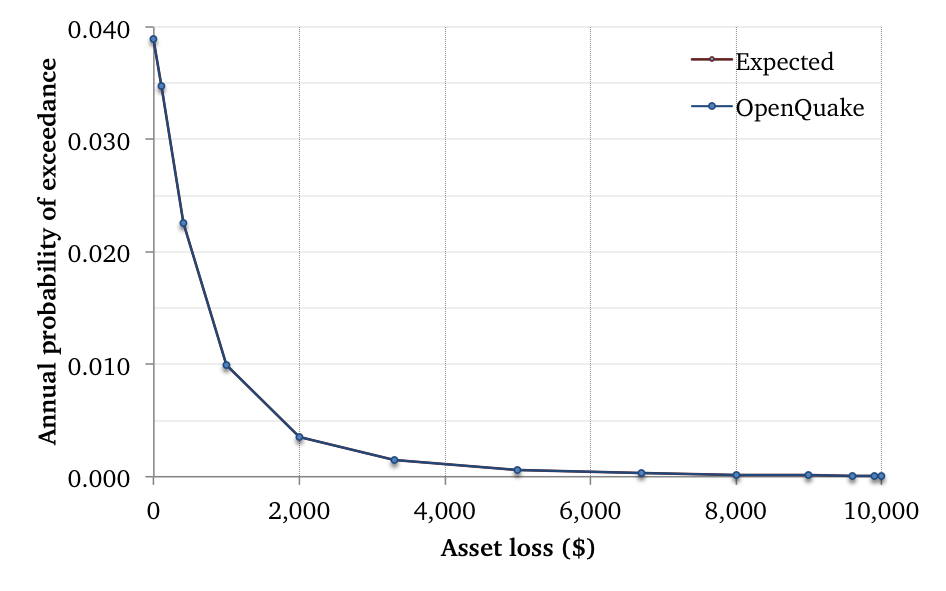
\includegraphics[width=12cm]{qareport/figures/fig-lc-cr-1c}
\caption{Loss curve comparison for classical risk test case 1c}
\label{fig:lc-cr-1c}
\end{figure}

The area under the annual loss exceedance curve gives the average annual loss.
\begin{table}[htbp]

\centering
\begin{tabular}{ l r r r }

\hline
\rowcolor{anti-flashwhite}
\bf{Result} & \bf{Expected} & \bf{OpenQuake} & \bf{Difference}\\
\hline
Average loss & 35.13 & 35.13 & 0\% \\
\hline
\end{tabular}

\caption{Results for classical risk test case 1c}
\label{tab:result-cr-1c}
\end{table}
Table~\ref{tab:result-cr-1c} shows the comparison of the OpenQuake result for average annual loss with the expected result.

% % % ---------------------------------------------------------------------------
\subsubsection{Case 1d}
This test case is identical to Case~1c described above, except for the use of the Beta distribution for the vulnerability functions instead of the lognormal distribution. The conditional loss ratio exceedance matrix in this case is populated by evaluating the complementary cumulative distribution function (CCDF) of the Beta distribution at each of the prescribed intensity levels, for the set of loss ratios.

\begin{table}[htbp]

\centering
\begin{tabular}{ l c c c c c c c c c }

\hline
\rowcolor{anti-flashwhite}
\bf{LR | PGA} & \bf{0.05g} & \bf{0.20g} & \bf{0.40g} & \bf{0.60g} & \bf{0.80g} & \bf{1.00g} & \bf{1.20g} & \bf{\dots} & \bf{2.00g} \\
\hline
\bf{0.01} & 0.496 & 1.000 & 1.000 & 1.000 & 1.000 & 1.000 & 1.000 & \dots & 1.000 \\
\bf{0.04} & 0.000 & 0.485 & 0.999 & 1.000 & 1.000 & 0.999 & 0.996 & \dots & 1.000 \\
\bf{0.10} & 0.000 & 0.000 & 0.472 & 0.959 & 0.984 & 0.987 & 0.982 & \dots & 1.000 \\
\bf{0.20} & 0.000 & 0.000 & 0.000 & 0.468 & 0.844 & 0.928 & 0.944 & \dots & 1.000 \\
\bf{0.33} & 0.000 & 0.000 & 0.000 & 0.032 & 0.473 & 0.778 & 0.871 & \dots & 1.000 \\
\bf{0.50} & 0.000 & 0.000 & 0.000 & 0.000 & 0.100 & 0.500 & 0.738 & \dots & 1.000 \\
\bf{0.67} & 0.000 & 0.000 & 0.000 & 0.000 & 0.006 & 0.222 & 0.563 & \dots & 0.999 \\
\bf{0.80} & 0.000 & 0.000 & 0.000 & 0.000 & 0.000 & 0.072 & 0.394 & \dots & 0.995 \\
\bf{0.90} & 0.000 & 0.000 & 0.000 & 0.000 & 0.000 & 0.013 & 0.234 & \dots & 0.976 \\
\bf{0.96} & 0.000 & 0.000 & 0.000 & 0.000 & 0.000 & 0.001 & 0.115 & \dots & 0.925 \\
\bf{0.99} & 0.000 & 0.000 & 0.000 & 0.000 & 0.000 & 0.000 & 0.038 & \dots & 0.822 \\
\bf{1.00} & 0.000 & 0.000 & 0.000 & 0.000 & 0.000 & 0.000 & 0.000 & \dots & 0.000 \\
\hline
\end{tabular}

\caption{Conditional loss ratio exceedance matrix for classical risk test case 1d}
\label{tab:lrem-bt-tax1-nzcov}
\end{table}

The loss ratio exceedance matrix in this case is shown in Table~\ref{tab:lrem-bt-tax1-nzcov}.

The loss curve thus calculated above is compared with the loss curve obtained using the OpenQuake classical PSHA based risk calculator in Figure~\ref{fig:lc-cr-1d}.

\begin{figure}[htbp]
\centering
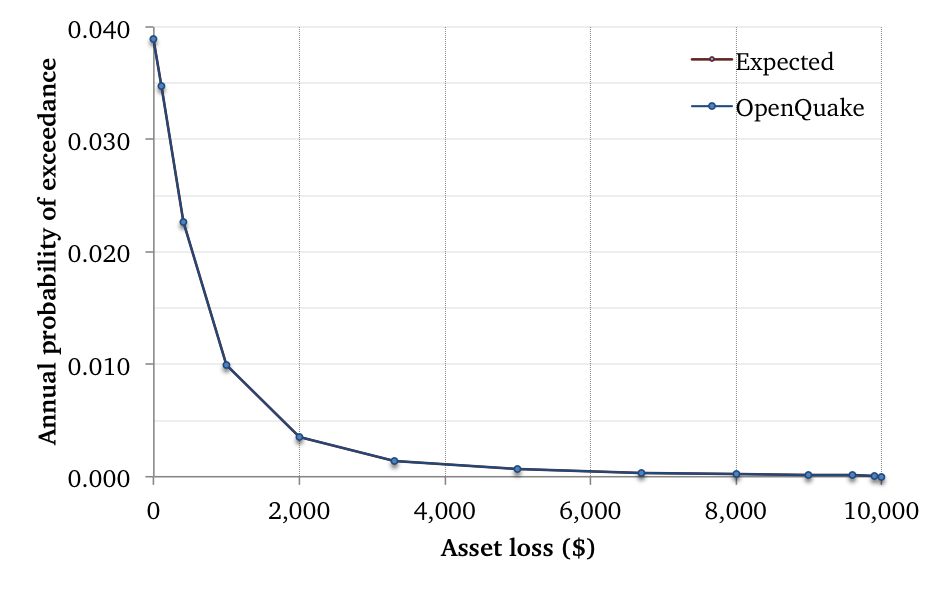
\includegraphics[width=12cm]{qareport/figures/fig-lc-cr-1d}
\caption{Loss curve comparison for classical risk test case 1d}
\label{fig:lc-cr-1d}
\end{figure}

The area under the annual loss exceedance curve gives the average annual loss.
\begin{table}[htbp]

\centering
\begin{tabular}{ l r r r }

\hline
\rowcolor{anti-flashwhite}
\bf{Result} & \bf{Expected} & \bf{OpenQuake} & \bf{Difference}\\
\hline
Average loss & 35.45 & 35.45 & 0\% \\
\hline
\end{tabular}

\caption{Results for classical risk test case 1d}
\label{tab:result-cr-1d}
\end{table}
Table~\ref{tab:result-cr-1d} shows the comparison of the OpenQuake result for average annual loss with the expected result.

% % % ---------------------------------------------------------------------------
\subsubsection{Case 1e}
This test case repeats the exercise from Case~1c using a vulnerability model with nonzero coefficients of variation, and using four `steps\_per\_interval'. Each interval between the loss ratios specified in the vulnerability model is further divided into four equal subdivisions, thus ensuring a greater number of loss values at which the exceedance curve will be computed. For instance, the interval between the loss ratios $[0.10, 0.20]$ is now subdivided into the following loss ratios: $[0.100, 0.125, 0.150, 0.175, 0.200]$.

The loss curve thus calculated above is compared with the loss curve obtained using the OpenQuake classical PSHA based risk calculator in Figure~\ref{fig:lc-cr-1e}.

\begin{figure}[htbp]
\centering
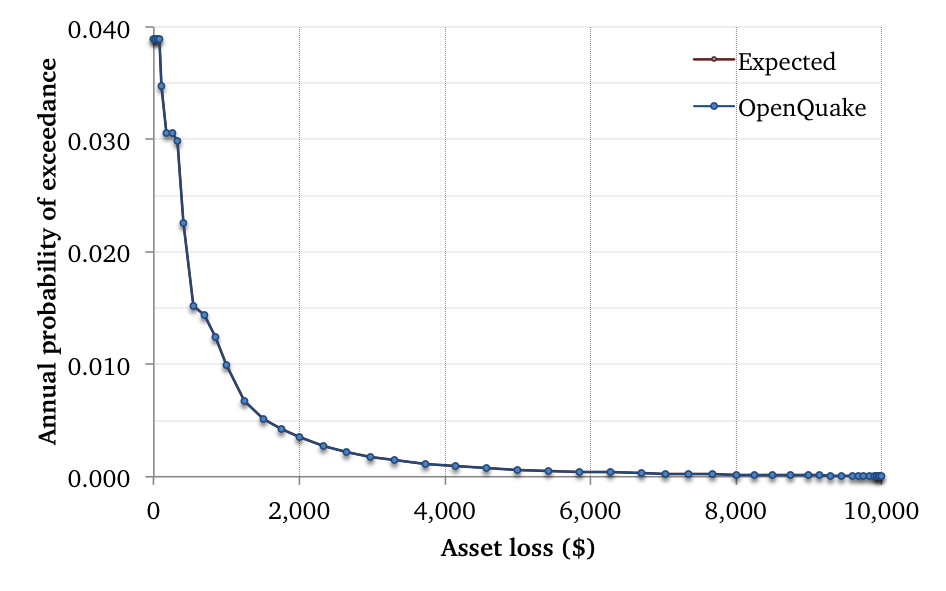
\includegraphics[width=12cm]{qareport/figures/fig-lc-cr-1e}
\caption{Loss curve comparison for classical risk test case 1e}
\label{fig:lc-cr-1e}
\end{figure}

The area under the annual loss exceedance curve gives the average annual loss.
\begin{table}[htbp]

\centering
\begin{tabular}{ l r r r }

\hline
\rowcolor{anti-flashwhite}
\bf{Result} & \bf{Expected} & \bf{OpenQuake} & \bf{Difference}\\
\hline
Average loss & 33.25 & 33.25 & 0\% \\
\hline
\end{tabular}

\caption{Results for classical risk test case 1e}
\label{tab:result-cr-1e}
\end{table}
Table~\ref{tab:result-cr-1e} shows the comparison of the OpenQuake result for average annual loss with the expected result.

% % % ---------------------------------------------------------------------------
\subsubsection{Case 2a}
In addition to computing direct structural losses, OpenQuake also provides support for computing losses incurred for the following other loss types:

\begin{itemize}
\item{Non-structural losses}
\item{Contents losses}
\item{Downtime, or business interruption losses}
\item{Occupant fatalities}
\end{itemize}

The purpose of this case is to test the calculation of the loss exceedance curve and average annual loss for the non-structural components of an asset. The replacement value of the non-structural components for the asset used in this case is $15,000$. Table~\ref{tab:vf-ln-tax1-nst} shows the mean loss ratios and corresponding coefficients of variation for the non-structural components vulnerability model used in this test case.

\begin{table}[htbp]

\centering
\begin{tabular}{ l r r r }

\hline
\rowcolor{anti-flashwhite}
\bf{Result} & \bf{Expected} & \bf{OpenQuake} & \bf{Difference}\\
\hline
Average loss & 63.48 & 63.48 & 0\% \\
\hline
\end{tabular}

\caption{Results for classical risk test case 2a}
\label{tab:result-cr-2a}
\end{table}
Table \ref{tab:result-cr-1b} shows the comparison of the OpenQuake result for average annual nonstructural loss with the expected result.

% % ---------------------------------------------------------------------------
\subsubsection{Case 2b}
The purpose of this case is to test the calculation of loss exceedance curve and average annual loss for the contents of an asset. The replacement value of the contents for the asset used in this case is $5,000$. Table~\ref{tab:vf-ln-tax1-con} shows the mean loss ratios and corresponding coefficients of variation in the contents vulnerability function used in this test case.
\begin{table}[htbp]

\centering
\begin{tabular}{ l r r r }

\hline
\rowcolor{anti-flashwhite}
\bf{Result} & \bf{Expected} & \bf{OpenQuake} & \bf{Difference}\\
\hline
Average loss & 59.60 & 59.60 & 0\% \\
\hline
\end{tabular}

\caption{Results for classical risk test case 2b}
\label{tab:result-cr-2b}
\end{table}
Table \ref{tab:result-cr-2b} shows the comparison of the OpenQuake result for average annual contents loss with the expected result.

% % ---------------------------------------------------------------------------
\subsubsection{Case 2c}
The purpose of this case is to test the calculation of loss exceedance curve and average annual loss for the downtime, or business-interruption losses for an asset. The loss due to downtime, or business-interruption for the asset used in this case is $2,000 / month$. Downtime losses are usually specified per unit time the asset will be unavailable for occupancy or use. Table~\ref{tab:vf-ln-tax1-dnt} shows the mean loss ratios and corresponding coefficients of variation for the downtime vulnerability function used in this test case.
\begin{table}[htbp]

\centering
\begin{tabular}{ l r r r }

\hline
\rowcolor{anti-flashwhite}
\bf{Result} & \bf{Expected} & \bf{OpenQuake} & \bf{Difference}\\
\hline
Average loss & 7.02 & 7.02 & 0.00\% \\
\hline
\end{tabular}

\caption{Results for classical risk test case 2c}
\label{tab:result-cr-2c}
\end{table}
Table \ref{tab:result-cr-2c} shows the comparison of the OpenQuake result for average annual downtime loss with the expected result.

% % ---------------------------------------------------------------------------
\subsubsection{Case 2d}
The purpose of this case is to test the calculation of the exceedance curve for fatalities and the average annual occupant fatalities for an asset. The number of occupants for the asset used in this case are 2 (day), 4 (transit), and 6 (night). An average value of 4 occupants is used for the calculation of the exceedance curve and average annual fatalities. Table~\ref{tab:vf-ln-tax1-dnt} shows the mean loss ratios and corresponding coefficients of variation for the occupants fatality vulnerability function used in this test case.
\begin{table}[htbp]

\centering
\begin{tabular}{ l r r r }

\hline
\rowcolor{anti-flashwhite}
\bf{Result} & \bf{Expected} & \bf{OpenQuake} & \bf{Difference}\\
\hline
Average annual fatalities & $2.91 \times 10^{-4}$ & $2.91 \times 10^{-4}$ & 0.00\% \\
\hline
\end{tabular}

\caption{Results for classical risk test case 2d}
\label{tab:result-cr-2d}
\end{table}
Table \ref{tab:result-cr-2d} shows the comparison of the OpenQuake result for average annual fatalities with the expected result.

% % % ---------------------------------------------------------------------------
% \subsubsection{Case 3a}
% The purpose of this case is to test the computation of the loss exceedance probabilities when the time period associated with the loss curve calculation is different from the time period associated with the hazard curve calculation. In this case, the hazard curve is calculated for a time period of 50 years, and the loss curve is calculated for a time period of 75 years.

Table~\ref{tab:vf-ln-tax1-nzcov} shows the mean loss ratios and corresponding coefficients of variation for the vulnerability function used in this test case.

\begin{table}[htbp]

\centering
\tabcolsep=0.11cm
\scalebox{0.6}{

\begin{tabular}{ l c c c c c c c c c c c }

\hline
\rowcolor{anti-flashwhite}
\bf{PGA} & \bf{0.05g} & \bf{0.20g} & \bf{0.40g} & \bf{0.60g} & \bf{0.80g} & \bf{1.00g} & \bf{1.20g} & \bf{1.40g} & \bf{1.60g} & \bf{1.80g} & \bf{2.00g} \\
\hline
\bf{P.O.E.} & 8.643\times10^{-1} & 7.171\times10^{-1} & 4.371\times10^{-1} & 2.364\times10^{-1} & 1.234\times10^{-1} & 6.427\times10^{-2} & 3.382\times10^{-2} & 1.802\times10^{-2} & 9.676\times10^{-3} & 5.192\times10^{-3} & 2.748\times10^{-3}\\
\hline
\end{tabular}

}

\caption{50-year hazard curve for PGA at a single site}
\label{tab:hc-l1-50}
\end{table}

The intensity levels for the hazard curve are extracted from the vulnerability function: $[0.05, 0.20, 0.40, 0.60, 0.80, 1.00, 1.20, 1.40, 1.60, 1.80, 2.00]$. The hazard curve gives the probabilities of exceedance for a set of intensity levels within a specified time period. The time period in this case, $t_H$, is fifty years. The hazard curve at the location of the single asset used in this test case is shown in Table~\ref{tab:hc-l1-50}.

The probabilities of exceedance are: $[8.643\times10^{-1}, 7.171\times10^{-1}, 4.371\times10^{-1}, 2.364\times10^{-1}, 1.234\times10^{-1}, 6.427\times10^{-2}, 3.382\times10^{-2}, 1.802\times10^{-2}, 9.676\times10^{-3}, 5.192\times10^{-3}, 2.748\times10^{-3}]$. The probabilities of exceedance are first converted to annual rates (or frequencies) of exceedance by employing the Poissonion conversion:

\begin{equation}
	\lambda(iml) = \frac{-\ln [1 - prob(IML > iml, t_H)]}{t_H}
\end{equation}

The annual frequencies of exceedance are: $[3.994\times10^{-2}, 2.525\times10^{-2}, 1.149\times10^{-2}, 5.394\times10^{-3}, 2.633\times10^{-3}, 1.329\times10^{-3}, 6.881\times10^{-4}, 3.636\times10^{-4}, 1.945\times10^{-4}, 1.041\times10^{-4}, 5.504\times10^{-5}]$.

The annual frequencies of occurrence are estimated by the differentiation of the annual frequencies of exceedance: $[1.469\times10^{-2}, 1.376\times10^{-2}, 6.101\times10^{-3}, 2.760\times10^{-3}, 1.305\times10^{-3}, 6.404\times10^{-4}, 3.245\times10^{-4}, 1.692\times10^{-4}, 9.035\times10^{-5}, 4.907\times10^{-5}]$.

The loss ratios at which the loss curve exceedance probabilities are calculated are obtained from the vulnerability function and the parameter `steps\_per\_interval'. The default value of `steps\_per\_interval' is one, which is the value used in this case. The loss ratios in the vulnerability function are $[0.01, 0.04, 0.10, 0.20, 0.33, 0.50, 0.67, 0.80, 0.90, 0.96, 0.99]$.

The vulnerability model is then transformed into a matrix describing probabilities of exceedance for the selected set of loss ratios conditional on the set of ground motion intensity levels. Since there is no variability in the loss ratio, calculation of the loss curves is straightforward in this case. Since the coefficients of variation in the vulnerability function are all zero, the lognormal distribution devolves into the degenerate distribution. The loss ratio exceedance matrix in this case is shown in Table~\ref{tab:lrem-ln-tax1-nzcov-75}.

\begin{table}[htbp]

\centering
\begin{tabular}{ l c c c c c c c c c }

\hline
\rowcolor{anti-flashwhite}
\bf{LR | PGA} & \bf{0.05g} & \bf{0.20g} & \bf{0.40g} & \bf{0.60g} & \bf{0.80g} & \bf{1.00g} & \bf{1.20g} & \bf{\dots} & \bf{2.00g} \\
\hline
\bf{0.01} & 0.494 & 1.000 & 1.000 & 1.000 & 1.000 & 1.000 & 1.000 & \dots & 1.000 \\
\bf{0.04} & 0.000 & 0.476 & 1.000 & 1.000 & 1.000 & 1.000 & 1.000 & \dots & 1.000 \\
\bf{0.10} & 0.000 & 0.000 & 0.453 & 0.980 & 0.999 & 1.000 & 1.000 & \dots & 1.000 \\
\bf{0.20} & 0.000 & 0.000 & 0.001 & 0.438 & 0.881 & 0.986 & 0.999 & \dots & 1.000 \\
\bf{0.33} & 0.000 & 0.000 & 0.000 & 0.039 & 0.427 & 0.812 & 0.959 & \dots & 1.000 \\
\bf{0.50} & 0.000 & 0.000 & 0.000 & 0.001 & 0.094 & 0.424 & 0.730 & \dots & 1.000 \\
\bf{0.67} & 0.000 & 0.000 & 0.000 & 0.000 & 0.017 & 0.170 & 0.427 & \dots & 1.000 \\
\bf{0.80} & 0.000 & 0.000 & 0.000 & 0.000 & 0.005 & 0.079 & 0.253 & \dots & 1.000 \\
\bf{0.90} & 0.000 & 0.000 & 0.000 & 0.000 & 0.002 & 0.043 & 0.162 & \dots & 0.999 \\
\bf{0.96} & 0.000 & 0.000 & 0.000 & 0.000 & 0.001 & 0.030 & 0.122 & \dots & 0.844 \\
\bf{0.99} & 0.000 & 0.000 & 0.000 & 0.000 & 0.001 & 0.025 & 0.106 & \dots & 0.494 \\
\bf{1.00} & 0.000 & 0.000 & 0.000 & 0.000 & 0.001 & 0.023 & 0.101 & \dots & 0.363 \\
\hline
\end{tabular}

\caption{Conditional loss ratio exceedance matrix for classical risk test case 3a}
\label{tab:lrem-ln-tax1-nzcov-75}
\end{table}

Now, the sum product of each row of the conditional loss ratio exceedance matrix with the annual frequencies of occurrence of the respective intensity levels gives the annual frequency of exceedance for the respective loss ratios. The loss ratio annual frequencies of exceedance thus calculated are: $[3.988\times10^{-2}, 3.617\times10^{-2}, 2.509\times10^{-2}, 1.280\times10^{-2}, 5.654\times10^{-3}, 2.765\times10^{-3}, 1.408\times10^{-3}, 7.772\times10^{-4}, 4.896\times10^{-4}, 3.276\times10^{-4}, 2.457\times10^{-4}, 2.037\times10^{-4}, 1.903\times10^{-4}]$.

The probabilities of exceedance of the set of loss ratios are obtained by converting the annual frequencies of exceedance back into probabilities of exceedance over 75 years by using the Poissonion equation. The loss curve probabilities of exceedance for a time period of 75 years are: $[9.498\times10^{-1}, 9.336\times10^{-1}, 8.477\times10^{-1}, 6.170\times10^{-1}, 3.456\times10^{-1}, 1.873\times10^{-1}, 1.002\times10^{-1}, 5.663\times10^{-2}, 3.606\times10^{-2}, 2.427\times10^{-2}, 1.826\times10^{-2}, 1.516\times10^{-2}, 1.417\times10^{-2}]$.

The loss curve thus calculated above is compared with the loss curve obtained using the OpenQuake classical PSHA based risk calculator in Figure~\ref{fig:lc-cr-3a}.

\begin{figure}[htbp]
\centering
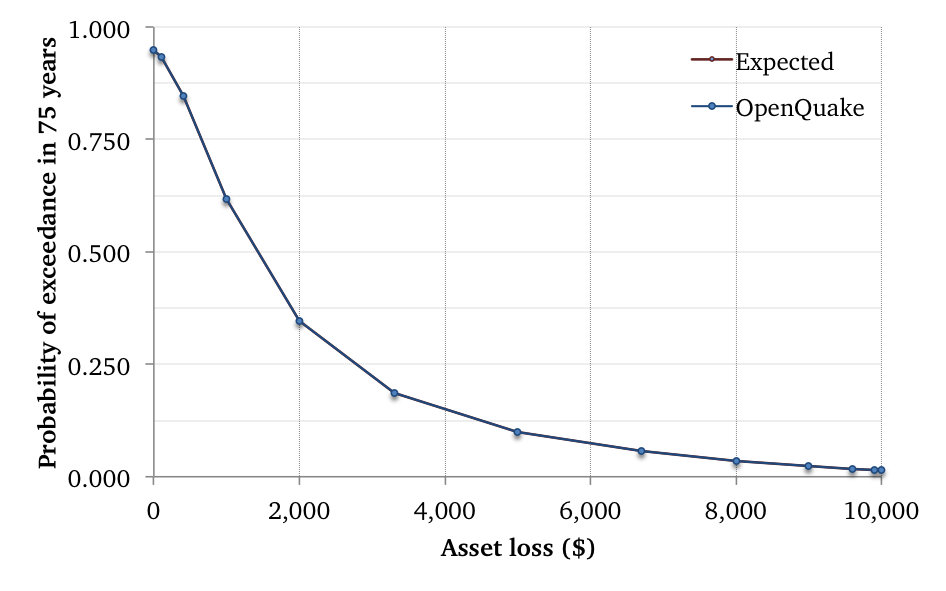
\includegraphics[width=12cm]{qareport/figures/fig-lc-cr-3a}
\caption{Loss curve comparison for classical risk test case 3a}
\label{fig:lc-cr-3a}
\end{figure}

The area under the loss exceedance curve gives the expected loss over 75 years.

% \input{qareport/results/tab-result-cr-3a}
% Table \ref{tab:result-cr-3a} shows the comparison of the OpenQuake result with the expected result.
% % % ---------------------------------------------------------------------------
% \subsubsection{Case 4a}
% There are several ways by which the replacement value of an asset can be specified in the exposure model. The different options are listed below:

\begin{itemize}
	\item Specify the aggregate value of each asset
	\item Specify the value per unit, and provide the number of units in each asset
	\item Specify the value per unit area, and provide the aggregate area of each asset
	\item Specify the value per unit area, specify the area per unit, and provide the number of units in each asset
\end{itemize}

This case tests the computation of the mean and standard deviation of the loss when the aggregate asset value is provided in the exposure model. The vulnerability function used is the same as in Case~1c and shown in Table~\ref{tab:vf-ln-tax1-nzcov}. The aggregate asset value in this case is $20,000$. The average annual loss in this case should be exactly twice the value calculated in Case~1c.
% \input{qareport/results/tab-result-cr-4a}
% Table \ref{tab:result-cr-4a} shows the comparison of the OpenQuake result with the expected result.
% % % ---------------------------------------------------------------------------
% \subsubsection{Case 4b}
% This case tests the computation of the loss exceedance curve and average annual loss when the value of the assets is specified per unit, and the number of units in each asset are provided in the exposure model. The vulnerability function used is the same as in Case~1c and shown in Table~\ref{tab:vf-ln-tax1-nzcov}. The asset has two units, and the value per unit is $7,500$. The aggregate asset value in this case is $15,000$.
% \input{qareport/results/tab-result-cr-4b}
% Table \ref{tab:result-cr-4b} shows the comparison of the OpenQuake result with the expected result.
% % % ---------------------------------------------------------------------------
% \subsubsection{Case 4c}
% This case tests the computation of the loss exceedance curve and average annual loss when the value of the assets is specified per unit area, and the aggregate area of each asset is provided in the exposure model. The vulnerability function used is the same as in Case~1c and shown in Table~\ref{tab:vf-ln-tax1-nzcov}. The asset has an aggregate area of $1,000$ sq. units, and the value per unit area is $5$. The aggregate asset value in this case is $5,000$. The average annual loss in this case should be exactly half the value calculated in Case~1c.
% \input{qareport/results/tab-result-cr-4c}
% Table \ref{tab:result-cr-4c} shows the comparison of the OpenQuake result with the expected result.
% % % ---------------------------------------------------------------------------
% \subsubsection{Case 4d}
% This case tests the computation of the loss exceedance curve and average annual loss when the value of the assets is specified per unit area, the area is specified per unit, and the number of units in each asset are provided in the exposure model. The vulnerability function used is the same as in Case~1c and shown in Table~\ref{tab:vf-ln-tax1-nzcov}. The asset has three units, the area per unit is $400$ sq. units, and the value per unit area is $10$. The aggregate asset value in this case is $12,000$.
% \input{qareport/results/tab-result-cr-4d}
% Table \ref{tab:result-cr-4d} shows the comparison of the OpenQuake result with the expected result.

